% !TEX root = ../thesis-example.tex
%
\chapter{Implementierung}
\label{sec:impl}

Dieses Kapitel behandelt die  Zielsetzungen, konkrete Planung und die Implementierung der RapidMiner-Erweiterung.

\section{Planung}
\label{sec:impl:plan}
Zuerst müssen wir betrachten, welche Begebenheiten die RapidMiner-Plattform uns bietet, d.h. welche Datentypen ein Parser annehmen muss, wie man Ergebnisse möglichst ohne Informationsverlust übergibt und Goldstandards richtig einliest.

\begin{figure}[htb]
	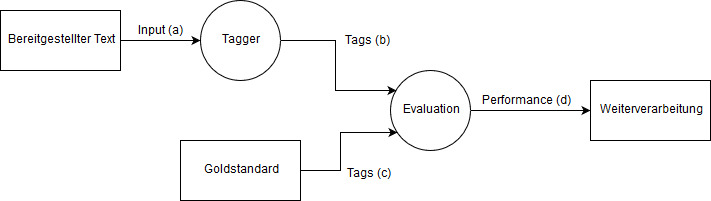
\includegraphics[width=\textwidth]{gfx/Dataflow.jpg}
	\caption{Datenfluss in einem typischen Tagging- und Evaluationsprozess}
	\label{fig:impl:overview}
\end{figure}

Eine Übersicht hierzu bietet Abbildung \ref{fig:impl:overview}, wobei insbesondere der Input (a) und Output (b) des Taggers interessant sind. Das Format des Goldstandards (c) ist exogen vorgegeben und das Ergebnis des Evaluationsprozesses muss lediglich RapidMiner-konform kodiert werden.

\subsection{Inputformat}
\label{sec:impl:plan:input}

Für die Eingabe an den Tagger wäre es optimal, wenn Outputs anderer Textverarbeitender RapidMiner-Erweiterungen, insbesondere vom \textit{Text Processing Plugin} :NC angenommen werden können. Hierzu kann einfach das Übergabeformat \textit{Document} aus diesem Plugin verwendet werden.

\subsection{Format für Tagger-Ergebnisse}
\label{sec:impl:plan:thru}

Für den Output eines Taggers macht es Sinn, zwei verschiedene Formatierungen zu betrachten: :TODO

\section{Conclusion}
\label{sec:system:conclusion}

